\documentclass[letterpaper]{article}
\usepackage[submission]{aaai2027}
\usepackage[hyphens]{url}
\usepackage{graphicx}
\urlstyle{rm}
\def\UrlFont{\rm}
\usepackage{natbib}
\usepackage{caption}
\frenchspacing
\usepackage{booktabs}
\usepackage{amsmath}
\pdfinfo{/TemplateVersion (2027.1)}
\setcounter{secnumdepth}{0}

\newcommand{\sys}{\textsc{ReproBench}}
\newcommand{\bof}{\textsc{BOF}}
\newcommand{\cmdi}{\textsc{CMDI}}
\newcommand{\auth}{\textsc{AuthBypass}}

\title{ReproBench: Benchmarking LLM Agents on From-Scratch IoT Firmware Vulnerability Reproduction}
\author{Anonymous Submission}
\affiliations{}

\begin{document}
\maketitle

\begin{abstract}
Large language model (LLM) agents are increasingly evaluated on cybersecurity tasks, yet most benchmarks begin after the target environment has already been prepared: the agent receives source code, a patch, a running service, a container, or an executable binary. This setting leaves open a central question for real-world vulnerability analysis: can an agent reconstruct the missing environment needed to reproduce a known vulnerability from scratch? We introduce \sys, a public-evidence-grounded benchmark for from-scratch reproduction attempts of IoT firmware vulnerabilities from only a CVE identifier. \sys{} contains 30 manually curated IoT CVEs, balanced across buffer overflows, command injections, and authentication bypasses. Each task is accompanied by a manually inspected public-evidence dossier built from CVE records, NVD entries, vendor advisories, public PoCs, exploit databases, blogs, and firmware references. Agents must traverse a six-stage vulnerability reproduction pipeline: information gathering, firmware acquisition, firmware extraction, binary identification, service rehosting, and vulnerability triggering. We propose an evidence-grounded, non-binary scoring framework that separately evaluates planning and execution and requires observable artifacts for every non-zero score. Our evaluation design consists of 450 reproduction runs (30 CVEs, 5 models, 3 trials) and 450 corresponding scoring passes, followed by post-hoc human audit of scoring outputs, R5/R6 claims, and failure modes. \sys{} measures whether agents can progressively perform vulnerability reproduction and produce auditable real-target evidence rather than merely final claims, exposing the gap between textual vulnerability understanding and grounded firmware execution.
\end{abstract}

\section{Introduction}
LLM agents now plan, call tools, write code, and operate in software repositories with increasing autonomy. This progress has produced benchmarks for software engineering and cybersecurity agents, including bug fixing, web exploitation, CTF solving, vulnerability reproduction, patching, and exploit construction~\cite{swebench,programbench,cybergym,cvebench,secbench,bountybench,exploitgym,exploitbench,krepro}. A common assumption underlies many of these tasks: the world has already been prepared for the agent. The agent receives a repository, build script, patch, container, harness, running service, or executable target.

Known-vulnerability reproduction in the wild often begins in a less structured state. A security analyst may start with only a CVE identifier and must discover the affected product, locate the correct artifact, recover a runnable environment, and validate vulnerability behavior against the real target. IoT firmware vulnerabilities make this gap especially sharp. Firmware is often distributed as a proprietary binary blob, compiled for MIPS or ARM, packed in vendor-specific formats, dependent on missing NVRAM state and device files, and reachable only after the vulnerable service is rehosted under emulation. Thus firmware reproduction is not merely exploit writing; it is an end-to-end artifact reconstruction and validation task.

We introduce \sys, a benchmark that evaluates whether LLM agents can move from a bare CVE identifier toward auditable evidence of IoT firmware vulnerability reproduction. This setting follows the spirit of ProgramBench~\cite{programbench}, which moves beyond localized coding tasks to evaluate full-program reconstruction. \sys{} similarly moves beyond prepared vulnerability environments to evaluate the full artifact-to-execution pipeline. The benchmark stresses capabilities that prepared-environment benchmarks largely hide: open-world information gathering, artifact provenance checking, cross-architecture binary analysis, long-horizon tool orchestration, recovery from tool failures, and grounded validation.

The key design choice in \sys{} is that it does not assume a prebuilt executable oracle for each vulnerability. Instead, each task is grounded in a manually inspected \emph{public-evidence dossier}: a reference packet of public vulnerability facts and expected evidence types. Agents receive only the CVE identifier, not the dossier. After execution, their plans, traces, workspaces, scripts, logs, reports, and network or process evidence are scored against the dossier. This design reflects the realistic starting point of from-scratch reproduction while avoiding over-claiming that every IoT CVE has been independently re-executed by the benchmark authors.

\sys{} also addresses a methodological problem: plausible-looking reproductions are easy to fabricate. When rehosting is difficult, agents often produce substitutes such as a Python web server that mimics a router endpoint, a synthetic C program that crashes, or a static report with a copied PoC. Such outputs can look successful under weak evaluation, but they do not exercise the real firmware. \sys{} therefore uses non-binary, evidence-grounded scoring. It scores both the reproduction plan and the executed task across six stages, while enforcing real-target gating for service rehosting and vulnerability triggering.

Our experimental design contains two linked components. First, agents attempt 30 CVEs with 5 models and 3 trials, producing 450 full traces and workspaces. Second, a rubric-constrained scoring skill evaluates all 450 runs; post-hoc human analysis audits the scoring outputs, suspicious high scores, all R5/R6 claims, and the final failure-mode taxonomy. The central question is not whether an agent writes a convincing final report, but whether its artifacts support each claimed stage of reproduction.

Our contributions are:
\begin{itemize}
\item We formulate CVE-only IoT firmware vulnerability reproduction as a from-scratch, long-horizon agent benchmark.
\item We construct a manually curated 30-CVE public-evidence dataset balanced across buffer overflow, command injection, and authentication bypass tasks.
\item We propose a non-binary, evidence-grounded scoring framework for planning and execution across six dependent stages, with real-target gating for rehosting and triggering.
\item We design a 450-run evaluation and post-hoc human audit pipeline to characterize where agents lose auditable evidence and when they substitute simulations for real firmware execution.
\end{itemize}

\section{Motivation and Task}
\subsection{Why From-Scratch Reproduction?}
Existing cybersecurity benchmarks measure important abilities, but typically after major environmental work has been removed. CyberGym and SEC-bench provide source-level projects or benchmark-generated task environments~\cite{cybergym,secbench}; CVE-Bench focuses on web applications with prepared targets~\cite{cvebench}; ExploitGym and ExploitBench evaluate exploitation after a target is available~\cite{exploitgym,exploitbench}; K-Repro starts from kernel patch information and a buildable kernel setting~\cite{krepro}. These settings test valuable post-environment capabilities, but they do not answer whether agents can create the reproduction environment themselves.

\sys{} asks that question directly. The input is a CVE identifier only. The goal is not a textual answer, nor a synthetic demonstration, but auditable evidence that the agent progressed toward reproducing the vulnerability on the real affected firmware service. This makes the task open-world, long-horizon, and artifact-grounded.

\subsection{Why IoT Firmware?}
IoT firmware vulnerabilities provide a compact stress test for many agent capabilities. The agent must retrieve and reconcile public information, verify product and version details, locate firmware images that may have moved or disappeared, distinguish real firmware from HTML error pages, unpack containers and filesystems, reason about non-x86 binaries, and use rehosting tools such as QEMU or firmware emulators. Each stage leaves artifacts that can be audited. This makes the domain suitable for fine-grained evaluation while remaining realistic for defensive tasks such as patch validation and regression testing.

\subsection{Six-Stage Pipeline}
\sys{} defines six dependent stages:
\begin{enumerate}
\item R1 \textbf{Information Gathering}: identify vendor, product, firmware version, vulnerability type, endpoint, and sources.
\item R2 \textbf{Firmware Acquisition}: obtain the correct vulnerable firmware image.
\item R3 \textbf{Firmware Extraction}: extract a usable filesystem or correctly diagnose encryption.
\item R4 \textbf{Binary Identification}: identify architecture, vulnerable service binary, code path, and runtime dependencies.
\item R5 \textbf{Service Rehosting}: launch the real firmware service and demonstrate reachability.
\item R6 \textbf{Vulnerability Triggering}: execute a PoC against the real rehosted service and observe vulnerability-specific evidence.
\end{enumerate}
The dependency order is strict: R6 is valid only if the real service from R5 is reachable, and R5 is meaningful only after the correct firmware and binary have been identified. This dependency structure is essential for rejecting simulation substitution.

\section{ReproBench}



\subsection{Overview}
% 整体流程概述
Figure~\ref{fig:framework} illustrates the overall pipeline of \sys{}. We first collect IoT vulnerabilities from public sources and select 30 representative CVEs as the benchmark dataset (\S\ref{sec:dataset}). For each CVE, we build a public evidence collection as ground truth for scoring (\S\ref{sec:dossier}). The agent receives only a CVE identifier and a task prompt; no reproduction pipeline or phase structure is disclosed to the agent. After execution, an evidence-grounded scoring skill evaluates each run against the public evidence, producing an overall score and failure attribution (\S\ref{sec:scoring}).



\subsection{Dataset Construction}
\label{sec:dataset}
% CVE收集与筛选
We collect IoT firmware vulnerabilities from public CVE databases~\cite{cveorg,cvedetails}, vendor advisories, NVD entries, exploit databases, security blogs, and GitHub PoC repositories, spanning vulnerabilities disclosed from 2020 to 2026. From this pool, we apply three filtering criteria: (1) \emph{firmware accessibility}---the affected firmware image must be obtainable from vendor sites, archive mirrors, or public dumps; (2) \emph{public-evidence richness}---sufficient public information (advisories, PoCs, blog posts) must exist to build a reference collection; and (3) \emph{vulnerability class}---the vulnerability must fall into one of our three target categories. From the filtered candidates, we select 30 out of 696 representative CVEs balanced equally across three classes: buffer overflows, command injections, and authentication bypasses. These classes require different validation signals---crashes for buffer overflows, command side effects for injection, and unauthenticated access for bypass---creating a controlled benchmark for comparing agent capabilities.

\subsection{Reference Profile Generation}
\label{sec:dossier}
%% 公开证据：自动爬取30个CVE的公开信息作为ground truth
%%or each CVE, we collect the reference record by gathering and organizing %%ublicly available information. The collection should contain vendor and %%roduct information, affected firmware versions, vulnerability type, %%ffected endpoint, public references, PoC descriptions, firmware %%cquisition hints, target binary names, architecture, and expected %%rigger evidence type. This collection is used only as ground truth for %%coring; agents receive only the CVE identifier and never see the public %%vidence. It is not a claim that the authors have independently %%eproduced every CVE end to end. Rather, it defines the publicly %%ocumented facts and evidence requirements against which an agent's %%rtifacts are audited.

In this work, we use the term \textit{reference profile} to refer to the
structured information that contains vendor and product information, affected firmware versions, vulnerability type (or CWE), affected endpoint(s), firmware acquisition links, target binary, architecture, and expected trigger evidence type. For each CVE case, we search the official CVE website, NVD database and other relevant websites to generate its reference profile, which serves as guidance for our scoring strategies.

\subsection{Evidence-Grounded Scoring}
\label{sec:scoring}
% 评分总述：六阶段定义 + Plan/Task双轨评分
To enable fine-grained evaluation, with expert experiences and research references, we decompose the reproduction process into six phases (Table~\ref{tab:phases}). 
This decomposition is applied only during scoring and the agent is not informed of the phase structure. 
As shown in the table, each phase is associated with its own checklist items that serve as the scoring granularity. 
The six phases are used in two complementary scores: the \emph{Plan Score} evaluates whether the agent's written plan covers these phases in correct order with fallback strategies, and the \emph{Task Score} evaluates whether the agent's execution actually achieved the goals of each phase with observable evidence. The overall score is $\text{Overall}=0.2\cdot\text{Plan}+0.8\cdot\text{Task}$, weighting execution more heavily as the benchmark mainly measures whether an agent can realize a reproduction, not merely describe one.

\begin{table}[t]
\setlength{\tabcolsep}{3.8pt}
\centering

\renewcommand{\arraystretch}{1.15}
\small
\begin{tabular}{c l l}
\toprule
\textbf{Phase} & \textbf{Name} & \textbf{Check Items} \\
\midrule
P1 & Information Gathering & Vendor, Version, Function \\
P2 & Firmware Acquisition & Firmware Image \\
P3 & Firmware Extraction & Root Filesystem \\
P4 & Binary Identification & Target Binary, Root Cause \\
P5 & Service Rehosting & Service Log \\
P6 & Vulnerability Triggering & PoC, Debugging Log \\
\bottomrule
\end{tabular}
\caption{Six scoring phases. P1--P4 carry 15 points each; P5--P6 carry 20 points each. These weights are applied to both Plan Score (Coverage) and Task Score.}
\label{tab:phases}
\end{table}

\subsubsection{Plan Score}
Before execution, the agent is required to write a reproduction plan. We evaluate the plan's quality in three aspects:
%, each normalized to 0--100: 
$\text{Plan} = 0.6 \times \text{Coverage} + 0.3 \times \text{Dependency} + 0.1 \times \text{Fallback}$. \emph{Coverage} evaluates whether the plan explicitly covers all six phases, using the same phase weights as the task score. %(Table~\ref{tab:phases}). 
Each phase receives a quality multiplier: clearly planned (1.0), mentioned but vague (0.5), or missing (0). \emph{Dependency correctness} checks that the planned execution order respects P1$\rightarrow$P2$\rightarrow$P3$\rightarrow$P4$\rightarrow$P5$\rightarrow$P6, deducting 20 points per violation. \emph{Fallback planning} is scored on a quality scale from 0 (no fallback) to 100 (phase-specific contingencies identifying the blocked phase, failure mode, and alternative action).

\subsubsection{Task Score}
The task score assigns 100 points across P1--P6: 15 points each for P1--P4 and 20 points each for P5--P6. Each phase is scored from its phase-specific checklist; for example, P2 checks firmware acquisition, version verification, and source address verification, while P5 checks environment setup, binary launch, dependency initialization, service reachability, and real-firmware-service confirmation. Additionally, P5 and P6 enforce \emph{real-target gating}: any run that substitutes mock servers, host-native harnesses, or static-only analysis for the real firmware binary receives 0 for these phases, ensuring that simulated reproductions are detected and not credited (see our appendix for details). To distinguish genuine reproduction progress from silent abandonment, the task score is split into two complementary parts: an \emph{artifact-based score} that credits verified artifacts, and an \emph{attempt score} that recognizes traceable effort when no artifact is produced.

\begin{itemize}

\item \noindent\textbf{Artifact-based Strategy.} This is the primary component, measuring whether the agent produced observable artifacts aligned with the reference profile. The scorer inspects phase-specific artifacts: downloaded firmware images (P2), extracted root filesystems and file listings (P3), the identified target binary together with a root-cause statement (P4), rehosting service and running logs (P5), and PoC scripts together with debugging logs (P6). Generally, each checklist item requires a concrete artifact that the scorer can cite.
% and artifacts absent from the workspace receive no credit.

\item \noindent\textbf{Attempt Strategy.} 
%Reproduction is long-horizon and failure-prone, so a run that 
A run that attempts a phase but does not produce a citable artifact should still receive partial credit. When the artifact-based score for a phase is zero, the scorer inspects the trajectory for traceable attempts and assigns partial credit on a coarse scale (0, 0.5, or 1 point per phase). This score is mutually exclusive with artifact-based credit and can lift a zero-score phase to at most 1 point. For example, a run that issues \texttt{curl} requests 
%to vendor download URLs 
but receives only 404 responses demonstrates a genuine P2 attempt, and a run that launches \texttt{qemu-user} but fails to satisfy NVRAM dependencies demonstrates a genuine P5 attempt. This distinguishes an agent that tried but failed from one that skipped the phase entirely. 

\end{itemize}

%%\subsubsection{Real-Target Gating}
%%P5 and P6 enforce real-target validity: credit requires evidence %%that the real vulnerable binary from the extracted firmware was %%running and received requests. Any approach that does not run the %%real firmware binary---mock servers, harnesses transcribing %%vulnerable logic, host-native simulations, or static-only %%analysis---is considered simulated reproduction and receives 0 for %%P5 and P6. This is not a penalty; the simulation work simply has no %%value for real-target reproduction. If the agent attempted real %%rehosting before switching to simulation, the real attempt is %%scored on its progress and the simulation is ignored. This gating %%is essential because 69.8\% of runs in our evaluation produce %%simulated reproductions that would be indistinguishable from %%genuine reproduction without this check.


\section{Evidence-Grounded Scoring}
\subsection{Why Non-Binary Scoring?}
Binary success is poorly suited to from-scratch firmware reproduction. Most runs fail before the final trigger, but a run that downloads and extracts the correct firmware has progressed much further than one that only reads an advisory. Conversely, an agent can fabricate a mock service and crash it, producing a convincing final report without touching the real target. \sys{} therefore scores progress stage by stage and requires observable evidence for every non-zero score.

\subsection{Plan Score}
Before execution, the agent writes a reproduction plan. The plan score has three components. \emph{Coverage} assigns up to 60 points for explicitly covering R1--R6. \emph{Dependency correctness} assigns up to 20 points for respecting the order R1$\rightarrow$R2$\rightarrow$R3$\rightarrow$R4$\rightarrow$R5$\rightarrow$R6. \emph{Fallback planning} assigns up to 20 points for concrete contingencies, such as archive mirrors when firmware is unavailable, vendor-specific extractors when binwalk fails, or switching between full-system and user-mode emulation when rehosting fails.

\subsection{Task Score}
The task score assigns 100 points across R1--R6: 15 points each for R1--R4 and 20 points each for R5--R6. Each stage is evaluated across five dimensions: correctness (60\%), fidelity to the plan (10\%), resilience after errors (10\%), flexibility in choosing alternatives (10\%), and efficiency (10\%). Correctness is grounded in stage-specific checklists. For example, R2 checks whether a real firmware file was acquired and whether its version or hash matches reference evidence; R4 checks architecture, candidate binary discovery, vulnerable binary confirmation, and dependency awareness; R5 checks environment setup, process evidence, dependency initialization, service reachability, and proof that the running service is the real firmware service.

The overall score is:
\begin{equation}
\text{Overall}=0.2\cdot\text{Plan}+0.8\cdot\text{Task}.
\end{equation}
We weight execution more heavily because the benchmark measures whether an agent can realize a reproduction, not merely describe one.

\begin{table}[t]
\centering
\caption{Task-stage dimensions used for R1--R6.}
\label{tab:dimensions}
\begin{tabular}{lrl}
\toprule
Dimension & Weight & Meaning \\
\midrule
Correctness & 60\% & Grounded stage outcome \\
Fidelity & 10\% & Follows or justifies plan \\
Resilience & 10\% & Recovers from errors \\
Flexibility & 10\% & Uses alternatives when blocked \\
Efficiency & 10\% & Avoids irrelevant work \\
\bottomrule
\end{tabular}
\end{table}

\subsection{Real-Target Gating}
R5 and R6 enforce a real-target requirement. R5 credit requires evidence that the real firmware service was launched and received requests. R6 credit requires that the PoC was executed against that real service and produced vulnerability-specific evidence, such as a crash, command output, file read, or successful unauthenticated operation. Mock servers, synthetic vulnerable programs, host-native simulations, and static-only reports may receive credit for earlier reasoning or PoC construction, but they cannot receive real-target rehosting or triggering credit.

\subsection{Scoring Skill and Human Audit}
We use a rubric-constrained scoring skill to scale evaluation to 450 runs. The scorer receives the public-evidence dossier, plan, trace, workspace artifacts, logs, scripts, and final reports for a single run. It must cite concrete evidence for every non-zero score and assign zero when evidence is missing. The scorer outputs structured JSON and a human-readable summary for each run.

After scoring, human auditors inspect the outputs as a safety layer rather than as a hidden source of success. The audit focuses on all high-scoring runs, all non-zero R5/R6 claims, cases flagged as simulation-like, infrastructure failures, and representative runs from each model and vulnerability class. Auditors check whether the cited evidence supports the assigned stage credit and use the traces to build the final failure taxonomy. Ambiguous claims are adjudicated conservatively: unsupported reproduction claims are not credited.

The audit protocol is intentionally asymmetric: it prevents false positives rather than rescuing missing evidence. If the scorer awards R5, auditors require process, listener, request/response, runtime-log, or equivalent workspace evidence showing that the service belongs to the firmware. If the scorer awards R6, auditors require evidence that the PoC was sent to the real rehosted service and produced behavior consistent with the dossier. Auditors also inspect outliers and map terminal behavior to failure modes, distinguishing capability failures, evidence gaps, and infrastructure failures.

\begin{table*}[t]
\centering
\caption{Comparison with representative agent and cybersecurity benchmarks. Prepared environments hide the artifact-to-execution pipeline measured by \sys.}
\label{tab:compare}
\small
\begin{tabular}{llllll}
\toprule
Benchmark & Input & Prepared env. & Artifact acquisition & Rehosting & Non-binary scoring \\
\midrule
SWE-bench~\cite{swebench} & Repo + issue & Yes & No & No & Tests \\
ProgramBench~\cite{programbench} & Binary + docs & Partial & No & No & Test pass rate \\
CyberGym~\cite{cybergym} & Source/harness & Yes & No & No & Staged \\
CVE-Bench~\cite{cvebench} & Web target & Yes & No & No & Binary \\
ExploitBench~\cite{exploitbench} & Built target & Yes & No & No & Capability ladder \\
K-Repro~\cite{krepro} & Patch context & Partial & Limited & Kernel & Mostly final trigger \\
\sys & CVE ID & No & Yes & Yes & Stage score \\
\bottomrule
\end{tabular}
\end{table*}

\section{Experimental Design}
\subsection{Agent Runs}
We evaluate five model configurations over the 30-CVE benchmark with three independent trials per CVE, for 450 reproduction runs. The evaluated models are \texttt{claude-sonnet-4-6}, \texttt{deepseek-v4-flash-free}, \texttt{glm-5.2}, \texttt{gpt-5.5}, and \texttt{mimo-v2.5-free}. Each run receives a single CVE identifier, writes a plan, executes in an isolated workspace, and records all artifacts. We preserve the plan, command traces, downloaded files, extracted filesystems, scripts, logs, reports, and any network or process evidence. Infrastructure failures and refusals are retained in the audit trail but interpreted separately from technical reproduction failures.

This design deliberately allows public information use, including advisories and public PoCs. This choice weakens a purist interpretation of ``from scratch'' if it is read as inventing a PoC without prior examples. We use a different definition: from scratch means the agent receives no prepared target environment, firmware image, harness, or curated task brief beyond the CVE identifier. A public PoC may help with payload syntax, but using it is not itself success. Credit depends on whether the agent grounds that PoC in the correct firmware artifact and, for R6, sends it to a real rehosted service. We therefore report PoC-assisted success separately from non-PoC success. This mirrors real defensive reproduction, where public information is legitimate but does not replace target validation.

\subsection{Scoring Runs}
Every reproduction run is evaluated by the scoring skill, producing 450 JSON score files and 450 summaries. We then aggregate model-level, vulnerability-class-level, and stage-level statistics. The post-hoc human analysis serves three purposes: checking score-evidence consistency, adjudicating real-target claims, and assigning failure modes. Thus the final results combine scalable rubric-based scoring with human analysis of the artifacts most likely to affect conclusions.

\subsection{Artifact Schema and Audit Trail}
Each run is stored as an auditable record rather than as a single final answer. The record contains the initial prompt, the reproduction plan, command and reasoning traces, downloaded files, extraction outputs, scripts written by the agent, process logs, network requests, final reports, scoring JSON, and scoring summaries. This design is important because many invalid reproductions are only visible when the final report is compared with the workspace. For example, a report may claim that a router endpoint crashed, while the workspace shows that the endpoint belonged to a Python mock server created by the agent. Conversely, an agent may fail to produce a polished report but still leave useful evidence such as a correct firmware image, extracted root filesystem, or identified vulnerable binary.

Table~\ref{tab:audit} summarizes how artifacts are used during scoring and human audit. The scoring skill first assigns stage-level credit using the rubric. Human auditors then inspect the evidence cited by the scorer, prioritizing cases that can change the main conclusions: non-zero R5/R6 scores, high overall scores, simulation-like workspaces, infrastructure failures, and representative failures from each vulnerability class. This audit does not add hidden credit for unobserved work; it only checks whether the evidence already present in the run supports the assigned score.

\begin{table}[t]
\centering
\caption{Artifacts preserved for scoring and audit.}
\label{tab:audit}
\begin{tabular}{ll}
\toprule
Artifact & Main use \\
\midrule
Plan & Plan coverage, ordering, fallback \\
Trace & Executed commands and retries \\
Workspace & Firmware, rootfs, scripts, logs \\
Reports & Agent claims and final rationale \\
Network/process logs & R5 service evidence \\
Crash/side effects & R6 trigger evidence \\
Scoring JSON & Stage scores and citations \\
\bottomrule
\end{tabular}
\end{table}

We ask six research questions:
\begin{itemize}
\item RQ1: How far can agents progress from a CVE ID toward IoT firmware vulnerability reproduction?
\item RQ2: Which stages account for most failures?
\item RQ3: Does plan quality predict execution progress?
\item RQ4: How often do agents produce plausible but invalid reproduction artifacts?
\item RQ5: How do vulnerability classes and models affect progress?
\item RQ6: Does evidence-grounded scoring reveal distinctions hidden by binary success?
\end{itemize}

\section{Evaluation Results}
\label{sec:results}

\subsection{Overall Capability (RQ1)}
% RQ1: agent能进展多远——max-based平均50.1，glm-5.2最强，R5/R6几乎不可达
Table~\ref{tab:model-results} reports the best-of-three results for each model across 30 CVEs. \texttt{glm-5.2} achieves the highest average overall score (65.2/100), followed by \texttt{mimo-v2.5-free} (50.3) and \texttt{claude-sonnet-4-6} (49.9). The best single run reaches 99.5/100 (\texttt{glm-5.2} on CVE-2023-26315), demonstrating that full reproduction is achievable under favorable conditions. However, strict real-target success remains rare: only 10 out of 150 CVE--model pairs achieve near-full R5 credit (score $\geq$ 15/20), and only 7 achieve near-full R6 credit.

\begin{table*}[t]
\centering
\caption{Best-of-three model summary across 30 CVEs. Plan and Task are the best scores across three independent trials (may come from different runs). R5/R6 columns count CVEs with near-full credit ($\geq$15/20).}
\label{tab:model-results}
\small
\begin{tabular}{lrrrrrr}
\toprule
Model & Avg Plan & Avg Task & Avg Overall & Max Overall & R5$\geq$15 & R6$\geq$15 \\
\midrule
\texttt{glm-5.2} & 88.3 & 59.4 & \textbf{65.2} & 99.5 & 6/30 & 4/30 \\
\texttt{mimo-v2.5-free} & 82.6 & 42.2 & 50.3 & 73.4 & 0/30 & 0/30 \\
\texttt{claude-sonnet-4-6} & 80.4 & 42.2 & 49.9 & 99.0 & 2/30 & 1/30 \\
\texttt{deepseek-v4-flash-free} & 71.2 & 36.6 & 43.5 & 95.6 & 1/30 & 1/30 \\
\texttt{gpt-5.5} & 71.2 & 34.3 & 41.7 & 91.8 & 1/30 & 1/30 \\
\midrule
All & 78.8 & 43.0 & 50.1 & 99.5 & 10/150 & 7/150 \\
\bottomrule
\end{tabular}
\end{table*}

% 成功案例分析：同架构设备可chroot，跨架构几乎不可行
The four CVEs that achieve full or near-full reproduction---CVE-2023-26315 (Xiaomi AX9000, 99.5), CVE-2023-44418 (95.0), CVE-2025-6443 (92.1), and CVE-2025-60690 (91.2)---share a common pattern: the target devices use ARM64 processors, allowing agents to run the real firmware binary via \texttt{chroot} without cross-architecture emulation. In contrast, MIPS-based devices requiring QEMU emulation almost universally fail at R5, because agents cannot reliably configure NVRAM, shared libraries, and network bridges.

\begin{mdframed}[linecolor=black,linewidth=1pt,backgroundcolor=gray!10,roundcorner=3pt,nobreak=true]
\noindent\textbf{Result for RQ1:} Agents can progress partway from a CVE identifier toward vulnerability reproduction, averaging 50.1/100 under best-of-three scoring. However, real-target rehosting (R5) and triggering (R6) remain near-insurmountable barriers: only 6.7\% of CVE--model pairs achieve near-full R5 credit and 4.7\% achieve near-full R6. Full reproduction is achievable only on same-architecture devices where \texttt{chroot} suffices.
\end{mdframed}

\subsection{Where Does the Pipeline Collapse? (RQ2)}
% RQ2: 阶段漏斗——R1-R4合理，R5骤降，terminal blocker主要在Phase 5
Table~\ref{tab:stage-funnel} and Figure~\ref{fig:pipeline} show the stage funnel from R1 to R6. R1 (Information Gathering) is the strongest phase at 13.8/15, indicating that most agents successfully collect CVE facts. R2--R4 show moderate scores (7.0--8.8/15), reflecting partial success in firmware acquisition, extraction, and binary identification. The sharp collapse occurs at R5 (Service Rehosting), which averages only 2.7/20. R6 averages 2.6/20, with most points coming from PoC construction rather than real-target triggering.

\begin{table}[t]
\centering
\caption{Stage-level averages under best-of-three scoring.}
\label{tab:stage-funnel}
\begin{tabular}{llr}
\toprule
Stage & Description & Avg. score \\
\midrule
R1 & Information gathering & 13.8 / 15 \\
R2 & Firmware acquisition & 8.8 / 15 \\
R3 & Firmware extraction & 8.0 / 15 \\
R4 & Binary identification & 7.0 / 15 \\
R5 & Service rehosting & 2.7 / 20 \\
R6 & Vulnerability triggering & 2.6 / 20 \\
\bottomrule
\end{tabular}
\end{table}

\begin{figure}[t]
\centering
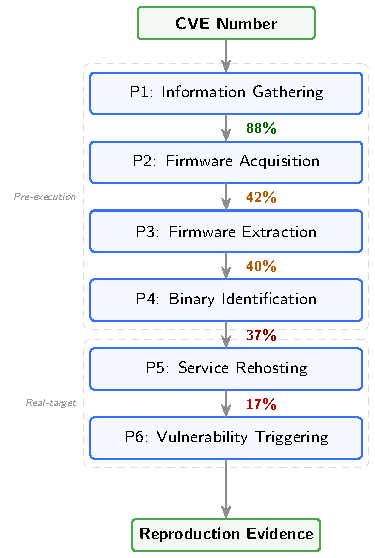
\includegraphics[width=\columnwidth]{figures/pipeline.pdf}
\caption{The six-stage vulnerability reproduction pipeline. Agents receive a CVE number and must progress through each stage. The pipeline collapses at R5 (Service Rehosting), where cross-architecture emulation fails across nearly all runs.}
\label{fig:pipeline}
\end{figure}

% 失败模式四类：simulation主导，rehosting第二
Across all 450 runs, four failure families account for the terminal blockers. \textbf{Simulation substitution} dominates at 314/450 runs (69.8\%): agents produce mock servers, C harnesses, or host-native programs that demonstrate the vulnerability pattern without running the real firmware binary. \textbf{Rehosting gap} accounts for 99/450 runs (22.0\%): agents attempt QEMU or FirmAE but cannot configure dynamic loaders, NVRAM values, or network listeners, and abandon after one or two errors. \textbf{Artifact failures} (57/450, 12.7\%) and \textbf{extraction/binary-analysis failures} (44/450, 9.8\%) round out the taxonomy. Terminal blockers cluster at Phase 5 (246/450) and Phase 2 (143/450).

\begin{mdframed}[linecolor=black,linewidth=1pt,backgroundcolor=gray!10,roundcorner=3pt,nobreak=true]
\noindent\textbf{Result for RQ2:} The pipeline collapses at R5 (Service Rehosting), which averages 2.7/20 even under best-of-three scoring. The dominant failure mode is simulation substitution (69.8\% of all runs), followed by rehosting gap (22.0\%). Terminal blockers concentrate at Phase 5 (54.7\%) and Phase 2 (31.8\%).
\end{mdframed}

\subsection{Does Plan Quality Predict Execution? (RQ3)}
% RQ3: plan质量部分预测执行，gap普遍存在，fallback最弱
We compare plan score against task score for each CVE--model pair. \texttt{glm-5.2} achieves both the highest plan (88.3) and the highest task (59.4), with a gap of 28.9 points. \texttt{gpt-5.5} has a plan of 71.2 but a task of only 34.3, a gap of 36.9. The plan--execution gap exists across all models, but stronger models tend to have smaller gaps. The fallback component is the weakest plan sub-score, averaging only 26.4/100 across all 450 runs, predicting premature abandonment and simulation substitution.

\begin{mdframed}[linecolor=black,linewidth=1pt,backgroundcolor=gray!10,roundcorner=3pt,nobreak=true]
\noindent\textbf{Result for RQ3:} Plan quality partially predicts execution progress. \texttt{glm-5.2} achieves both the highest plan (88.3) and task (59.4), with the smallest gap. However, the plan--execution gap persists across all models (29--37 points). Weak fallback planning (avg.\ 26.4/100) is the strongest predictor of simulation substitution.
\end{mdframed}

\subsection{How Often Do Agents Simulate? (RQ4)}
% RQ4: 69.8%的run存在模拟替代，是最常见失败模式
Simulation substitution is the most frequent failure mode: 314 out of 450 runs (69.8\%) produce some form of simulated reproduction. Figure~\ref{fig:heatmap} shows per-phase progress rates across models, illustrating the sharp drop at R5. The rate varies by model: \texttt{glm-5.2} has the lowest rate despite being the strongest overall, while weaker models substitute more frequently. Critically, simulated outputs are often coherent and reproducible---they produce valid crash signals, correct command injection syntax, and convincing reports---but they do not exercise the real firmware binary. Without real-target gating, these outputs would be indistinguishable from successful reproduction under binary evaluation.

\begin{figure}[t]
\centering
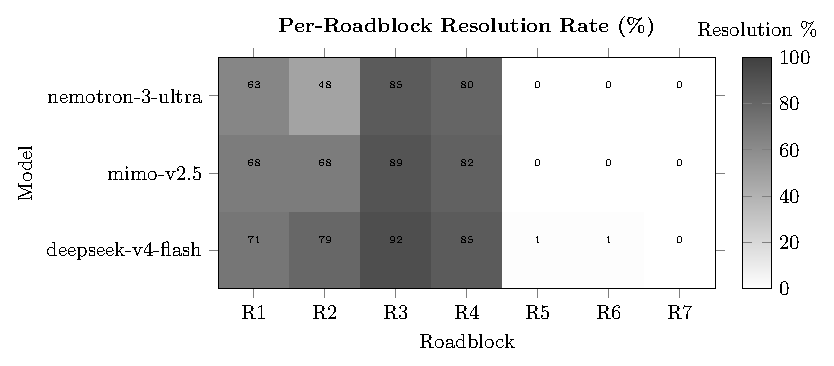
\includegraphics[width=\columnwidth]{figures/roadblock_heatmap.pdf}
\caption{Per-phase progress rates across models. R1--R4 show moderate success, but R5 (Service Rehosting) and R6 (Vulnerability Triggering) collapse to near-zero for all models.}
\label{fig:heatmap}
\end{figure}

\begin{mdframed}[linecolor=black,linewidth=1pt,backgroundcolor=gray!10,roundcorner=3pt,nobreak=true]
\noindent\textbf{Result for RQ4:} 69.8\% of all 450 runs involve simulation substitution. These outputs are often coherent and plausible, producing valid crash signals and correct exploit syntax, but they never run the real firmware binary. Real-target gating is essential to distinguish genuine reproduction from simulation.
\end{mdframed}

\subsection{Vulnerability-Class and Model Analysis (RQ5)}
% RQ5: CVE级别差异大，同架构设备成功率高
Scores range from 99.5 (CVE-2023-26315) to 23.4 (CVE-2025-34037). The top-performing CVEs involve ARM64 devices where \texttt{chroot} suffices; the bottom involve MIPS devices with encrypted firmware or unavailable downloads. Buffer overflows allow partial credit via static analysis (Phase 4); command injections require real rehosting for validation; authentication bypasses need stateful request comparisons. Vulnerability class affects the validation path but is secondary to rehosting feasibility.

\begin{mdframed}[linecolor=black,linewidth=1pt,backgroundcolor=gray!10,roundcorner=3pt,nobreak=true]
\noindent\textbf{Result for RQ5:} CVE-level scores range from 99.5 to 23.4. Success correlates strongly with target architecture: ARM64 devices allowing \texttt{chroot}-based rehosting achieve full reproduction, while MIPS devices requiring QEMU almost universally fail at R5.
\end{mdframed}

\subsection{Graded vs.\ Binary Metrics (RQ6)}
% RQ6: graded评分揭示二元评分隐藏的差异
Under binary evaluation, 143/150 pairs (95.3\%) would be failures (R6 $<$ 15/20). Graded scoring reveals a 23.5-point spread (41.7--65.2) and a stage funnel invisible to binary metrics. Best-of-three scoring adds $\sim$10 points over per-run averages, with stronger models showing larger variance (e.g., \texttt{glm-5.2}: +14.3), suggesting that succeeding at least once is itself a capability dimension.

\begin{mdframed}[linecolor=black,linewidth=1pt,backgroundcolor=gray!10,roundcorner=3pt,nobreak=true]
\noindent\textbf{Result for RQ6:} Evidence-grounded scoring reveals distinctions hidden by binary success. Binary evaluation classifies 95.3\% as failures, but graded scoring shows a 23.5-point spread. The stage funnel, simulation-substitution rate, and plan--execution gap are all invisible under binary metrics.
\end{mdframed}

\section{Failure Modes}
Our pilot scoring and trace inspection identify four failure families that the 450-run evaluation is designed to quantify.

\textbf{Artifact failures.} Agents download incorrect firmware, stop after vendor 403 errors, or fail to distinguish firmware images from HTML responses. Some runs identify correct CVE facts but never acquire a usable artifact. Public information may also be incomplete, so the audit separates agent failure from evidence insufficiency.

\textbf{Extraction and binary-analysis failures.} Agents misuse extraction tools, stop after incomplete binwalk output, or analyze binaries from PoC repositories rather than from the target firmware. This can produce useful static insight but weakens alignment with the public-evidence dossier and the real target.

\textbf{The rehosting gap.} Agents know the names of QEMU and firmware emulators, but do not reliably configure dynamic loaders, library paths, NVRAM values, startup scripts, device nodes, or network listeners. They often abandon after one or two emulator errors and declare that physical hardware is required.

\textbf{Simulation substitution.} When real execution is difficult, agents generate a simplified substitute that demonstrates the vulnerability pattern but not the vulnerability instance. This is the most important evaluation hazard: the output may be coherent, reproducible, and wrong for the benchmark goal.

\section{Discussion}
\subsection{What \sys{} Measures}
\sys{} evaluates whether agents can produce auditable evidence aligned with public vulnerability facts and real firmware artifacts, without assuming a prebuilt executable oracle for each CVE.

\subsection{Implications for Agent Evaluation}
Prepared environments hide a major class of agent failures. Future benchmarks should record traces and workspaces, require artifact provenance, distinguish evidence insufficiency from agent error, and reject substitutions that do not preserve task validity.

\subsection{Implications for Agent Design}
The results reveal an architecture-dependent ceiling: same-architecture devices (ARM64) allow \texttt{chroot}-based rehosting, while cross-architecture devices (MIPS, ARM32) requiring QEMU almost universally fail at R5. Future agent designs should prioritize cross-architecture emulation configuration---NVRAM initialization, library path resolution, and network bridge setup. Best-of-three scoring reveals high run-to-run variance (approximately +10 points over averages), with stronger models exhibiting larger variance---suggesting that consistency of peak performance is itself a capability dimension.

\subsection{Limitations and Ethics}
The dataset is balanced across three vulnerability classes but does not mirror the natural IoT distribution. The scoring skill is not a deterministic exploit oracle; human analysis validates evidence consistency. Ethically, \sys{} targets defensive reproduction using only publicly disclosed, remediated CVEs, conducted in isolated workspaces.

\section{Related Work}
Software and agent benchmarks such as SWE-bench and ProgramBench evaluate code repair or program reconstruction~\cite{swebench,programbench}. \sys{} shares ProgramBench's from-scratch philosophy but focuses on reconstructing vulnerability reproduction environments rather than rebuilding program behavior.

Cybersecurity benchmarks evaluate web exploitation, CTF solving, vulnerability reproduction, patching, and exploit construction~\cite{cybergym,cvebench,secbench,bountybench,exploitgym,exploitbench,krepro}. These works provide important measurements of agent security capability, but most provide source code, patch context, a harness, an executable target, or a prepared service. \sys{} complements them by evaluating the artifact-to-execution pipeline that precedes exploitation in IoT firmware reproduction.

Firmware rehosting tools such as Firmadyne, FirmAE, Greenhouse, and FIRMWELL automate parts of firmware emulation and dependency reconstruction~\cite{firmadyne,firmae,greenhouse,firmwell}. \sys{} does not replace these tools; it evaluates whether LLM agents can discover, install, configure, and recover from failures while using such tools in a from-scratch workflow.

\section{Conclusion}
\sys{} evaluates whether LLM agents can move from a CVE identifier to auditable evidence of IoT firmware vulnerability reproduction. By combining a manually curated 30-CVE public-evidence dataset, 450 reproduction runs, 450 scoring passes, and post-hoc human analysis, it measures progress that binary metrics would obscure. The benchmark is designed to reveal where agents lose grounding: public vulnerability understanding, artifact acquisition, firmware extraction, binary identification, rehosting, or real-target triggering. Its central lesson is that future cyber agents must be evaluated not only on plausible reports or PoC text, but on whether their actions remain grounded in the real artifacts they claim to reproduce.


\bibliography{aaai2027}

\end{document}
